\fig{fv:k5:plates}{两个接触点分别给出速度约束，平动与自转由联立确定}{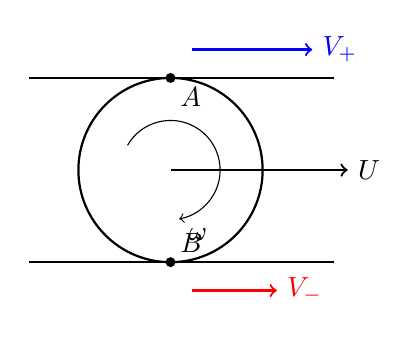
\begin{tikzpicture}[scale=.9]
\draw[thick](-2,1.3)--(2.3,1.3) (-2,-1.3)--(2.3,-1.3);\draw[thick](0,0)circle(1.3);
\fill(0,1.3)circle(2pt)node[below right]{$A$};\fill(0,-1.3)circle(2pt)node[above right]{$B$};
\draw[->,blue,thick](.3,1.7)--(2,1.7)node[right]{$V_+$};\draw[->,red,thick](.3,-1.7)--(1.5,-1.7)node[right]{$V_-$};
\draw[->,thick](0,0)--(2.5,0)node[right]{$U$};\draw[->](150:.7)arc(150:-80:.7)node[below right]{$\omega$};
\end{tikzpicture}}
图\ref{fv:k5:plates}中顺时针转动在 $A$处贡献向右的 $r\omega$，在 $B$处贡献向左的 $r\omega$。这就是两条速度式符号相反的几何原因。相加消去转动，相减消去平动：上下板同速只产生平动，等大反向则圆心静止而自转。若只有一处无滑动，便只有一个方程，不能只用几何约束同时确定 $U,\omega$。
